\documentclass{article}
\usepackage[margin = 0.15in,landscape]{geometry}
\usepackage{multicol}
\usepackage{array}
\usepackage{amsmath}
\usepackage{amssymb}
\usepackage{lmodern}
\usepackage{graphicx}

\setlength\parindent{0pt}
\renewcommand{\baselinestretch}{0.5}


\begin{document}
\begin{multicols*}{3}
    \subsection*{Two-Body Problem}
    Newton's Law: $\Sigma \vec{F}=\frac{d(m\vec{v})}{dt}=m\vec{a}$ \par
    Universal Law of Gravitation: $\vec{F}_g=-\frac{Gm_1m_2}{r^2}\frac{\vec{r}}{|\vec{r}|}$\par 
    Apply Newton's Laws to a two-body problem with the assumptions:
    \begin{enumerate}
        \itemsep0em
        \item Only system force: Gravity $\rightarrow$ acts along the line joining the centers of the bodies.
        \item Mass of each body is constant.
        \item Treat each body as a spherically symmetrical point mass with uniform density.
    \end{enumerate}
    Orbital Properties:
    \begin{itemize}
        \itemsep0em
        \item a = semimajor axis
        \item b = semiminor axis
        \item p = semiperimeter
        \item $r_a/r_p$ = radii of apoapsis/periapsis
        \item $\vec{e}$ = eccentricity
    \end{itemize}
    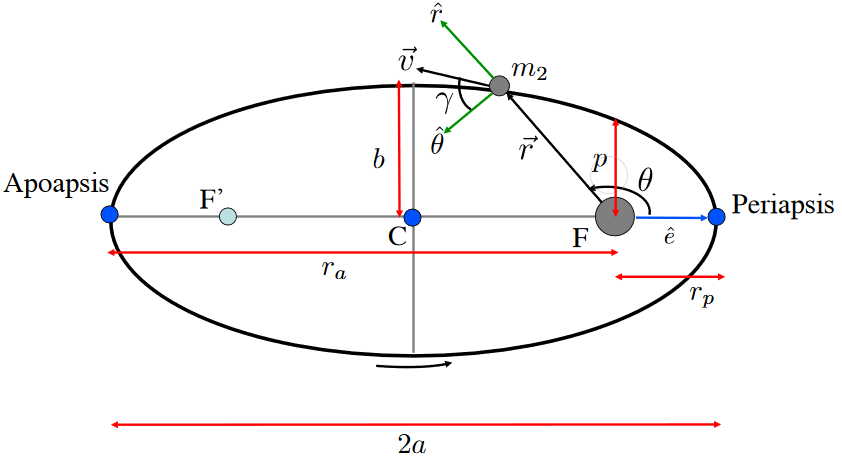
\includegraphics[width=\linewidth]{Figures/orbital_properties.png}
    Useful Equations:\par
    $a = \frac{1}{2}(r_a+r_p)$\par 
    $p=\frac{b^2}{a}=a(1-e^2)=\frac{h^2}{\mu}$\par 
    $r_a = \frac{p}{1-e}=a(1+e)$\par 
    $r_p = \frac{p}{1+e}=a(1-e)$\par
    $e = \frac{r_a-r_p}{r_a+r_p}$ = $\frac{c}{a}$ = $\frac{\sqrt{a^2-b^2}}{a}$ = $\sqrt{1+\frac{2h^2\varepsilon}{\mu^2}}$\par 
    $b = a\sqrt{1-e^2}$ \par
    Angular Momentum: $\vec{h} = \vec{r} \times \vec{v}$ = $\sqrt{\mu a (1-e^2)}$ \par
    Eccentricity Vector: $\vec{e} = \frac{\vec{v} \times \vec{h}}{\mu}-\frac{\vec{r}}{r}$\par
    Specific Energy: $\varepsilon = \frac{v^2}{2}-\frac{\mu}{r}$ = $\frac{\mu^2(e^2-1)}{2h^2}$\par
    \begin{itemize}
        \itemsep0em
        \item $\varepsilon < 0$ Motion of Body 2 is bounded wrt Body 1
        \item $\varepsilon \ge 0$ Motion of Body 2 is unbounded wrt Body 1
    \end{itemize}
    Conic Equation: $r = \frac{h^2/\mu}{1+e\cos{\theta}}$ = $\frac{p}{1+e\cos{\theta}}$\par 
    Vis-Viva Equation: $v=\sqrt{\frac{2\mu}{r}-\frac{\mu}{a}}$\par 
    True Anomaly:
\end{multicols*}  



\end{document}